Un maire souhaite végétaliser sa ville. Pour cela, il décide de planter des mûriers platanes dans les différents parcs.

Ces arbres sont réputés pour leurs qualités d'ombrage et de résistance à la sécheresse.

\subsection*{Partie A}

Au moment de la plantation, un mûrier platane mesure 1 mètre.

On suppose que chaque année la hauteur de l'arbre augmente de 40 cm.

Pour tout entier naturel $n$, on note $u_n$ la hauteur de l'arbre, en mètres, $n$ années après sa plantation. Ainsi $u_0=1$.

\begin{enumerate}
\item \begin{enumerate}
\item Calculer $u_1$.
\item Quelle sera la hauteur de l'arbre deux années après sa plantation ?
\end{enumerate}
\item Quelle est la nature de la suite $(u_n)$ ? Justifier.
\item Pour tout entier naturel $n$, exprimer $u_n$ en fonction de $n$.
\item Au bout de combien d'années le mûrier atteindra-t-il 9 mètres de haut ?
\end{enumerate}


\subsection*{Partie B}

Au moment de la plantation, l'arbre possède un tronc et deux branches.

Un an après la plantation, on observe 4 nouvelles branches.

Deux ans après la plantation, on observe 8 nouvelles branches.

Chaque année, le nombre de nouvelles branches double comme représenté sur le schéma ci-dessous :

\begin{center}
	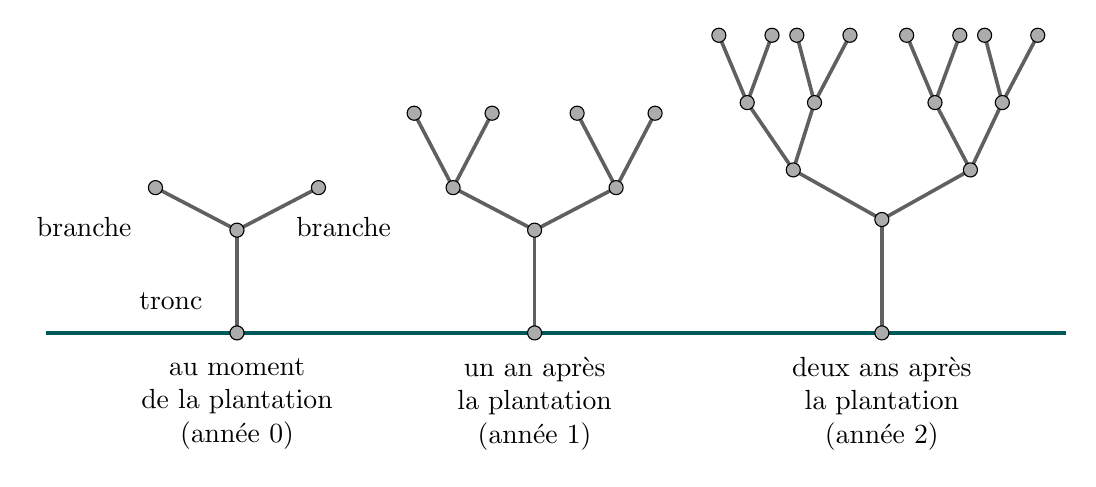
\begin{tikzpicture}[
		scale=0.9,
		point/.style={circle, draw=black, fill=gray!65, inner sep=1.8pt},
		branche/.style={line width=1.3pt, gray!75!black},
		sol/.style={line width=1.2pt, teal!70!black}
		]
		
		
		\draw[sol] (-1.7,0) -- (12.7,0);
		
		
		
		
		\coordinate (T0) at (1,0);
		\coordinate (N0) at (1,1.45);
		\coordinate (G0) at (-0.15,2.05);
		\coordinate (D0) at (2.15,2.05);
		
		\draw[branche] (T0) -- (N0);
		\draw[branche] (N0) -- (G0);
		\draw[branche] (N0) -- (D0);
		
		\node[point] at (T0) {};
		\node[point] at (N0) {};
		\node[point] at (G0) {};
		\node[point] at (D0) {};
		
		\node[left] at (-0.35,1.5) {branche};
		\node[right] at (1.7,1.5) {branche};
		\node[left] at (0.65,0.45) {tronc};
		
		\node[align=center] at (1,-1) {au moment\\de la plantation\\(année 0)};
		
		
		
		
		\coordinate (T1) at (5.2,0);
		\coordinate (N1) at (5.2,1.45);
		\coordinate (G1) at (4.05,2.05);
		\coordinate (D1) at (6.35,2.05);
		\coordinate (GG1) at (3.5,3.1);
		\coordinate (GD1) at (4.6,3.1);
		\coordinate (DG1) at (5.8,3.1);
		\coordinate (DD1) at (6.9,3.1);
		
		\draw[branche] (T1) -- (N1);
		\draw[branche] (N1) -- (G1);
		\draw[branche] (N1) -- (D1);
		\draw[branche] (G1) -- (GG1);
		\draw[branche] (G1) -- (GD1);
		\draw[branche] (D1) -- (DG1);
		\draw[branche] (D1) -- (DD1);
		
		\foreach \P in {T1,N1,G1,D1,GG1,GD1,DG1,DD1}
		{
			\node[point] at (\P) {};
		}
		
		\node[align=center] at (5.2,-1) {un an après\\la plantation\\(année 1)};
		
		
		
		
		\coordinate (T2) at (10.1,0);
		\coordinate (N2) at (10.1,1.6);
		
		\coordinate (G2) at (8.85,2.3);
		\coordinate (D2) at (11.35,2.3);
		
		\coordinate (GG2) at (8.2,3.25);
		\coordinate (GD2) at (9.15,3.25);
		\coordinate (DG2) at (10.85,3.25);
		\coordinate (DD2) at (11.8,3.25);
		
		\coordinate (A2) at (7.8,4.2);
		\coordinate (B2) at (8.55,4.2);
		\coordinate (C2) at (8.9,4.2);
		\coordinate (D2top) at (9.65,4.2);
		
		\coordinate (E2) at (10.45,4.2);
		\coordinate (F2) at (11.2,4.2);
		\coordinate (G2top) at (11.55,4.2);
		\coordinate (H2) at (12.3,4.2);
		
		\draw[branche] (T2) -- (N2);
		\draw[branche] (N2) -- (G2);
		\draw[branche] (N2) -- (D2);
		
		\draw[branche] (G2) -- (GG2);
		\draw[branche] (G2) -- (GD2);
		\draw[branche] (D2) -- (DG2);
		\draw[branche] (D2) -- (DD2);
		
		\draw[branche] (GG2) -- (A2);
		\draw[branche] (GG2) -- (B2);
		\draw[branche] (GD2) -- (C2);
		\draw[branche] (GD2) -- (D2top);
		
		\draw[branche] (DG2) -- (E2);
		\draw[branche] (DG2) -- (F2);
		\draw[branche] (DD2) -- (G2top);
		\draw[branche] (DD2) -- (H2);
		
		\foreach \P in {T2,N2,G2,D2,GG2,GD2,DG2,DD2,A2,B2,C2,D2top,E2,F2,G2top,H2}
		{
			\node[point] at (\P) {};
		}
		
		\node[align=center] at (10.1,-1) {deux ans après\\la plantation\\(année 2)};
		
	\end{tikzpicture}
\end{center}

Pour tout entier naturel $n$, on note $v_n$ le nombre de nouvelles branches $n$ années après la plantation. À la plantation, l'arbre possède 2 branches, ainsi on pose $v_0=2$.

\begin{enumerate}
\item Quelle est la nature de la suite $(v_n)$ ? Justifier.
\item \begin{enumerate}
\item Un an après la plantation, l'arbre a produit 4 nouvelles branches. Il possède alors un nombre total de branches égal à 6.

Montrer que, trois ans après sa plantation, l'arbre possède un nombre total de branches égal à 30.
\item On donne le programme ci-contre écrit en langage Python :

\begin{minipage}[t]{0.48\linewidth}
\emph{Rappel :} \texttt{for i in range(n)} permet de répéter $n$ fois un ensemble d'instructions.
\end{minipage}\hfill
\begin{minipage}[t]{0.42\linewidth}
\fbox{\begin{minipage}{0.9\linewidth}\ttfamily
v = 2\par
total = 2\par
for i in range(10):\par
\quad v = 2 * v\par
\quad total = total + v\par
print(total)
\end{minipage}}
\end{minipage}

La valeur affichée par ce programme est 4 094.

Dans le contexte de l'exercice, que représente la valeur 4 094 affichée par ce programme ?
\end{enumerate}
\end{enumerate}

\clearpage
